%&pdflatex
\documentclass[11pt]{article}

\usepackage{geometry}                % See geometry.pdf to learn the layout options. There are lots.
\geometry{letterpaper}                   % ... or a4paper or a5paper or ...
\usepackage{graphicx}
\usepackage{longtable}

\setlength{\parindent}{0pt}
\setlength{\parskip}{\baselineskip}%

\title{Programming Practice (PRP), Coursework Exercise 3 (33\%, 30 marks)}
%\author{Martin Chapman (martin.chapman@kcl.ac.uk)}
\date{}                                           % Activate to display a given date or no date

\begin{document}
\maketitle
%\section{}
%\subsection{}

\textbf{Please read the document marked `Continuous Assessment Guidelines' carefully, before attempting any piece of coursework.}

\emph{This assignment counts for 33\% of your mark for PRP continuous assessment, and is the third of four. If you have not yet completed the first two assignments for PRP, you are advised to do so before proceeding with this one.}

\emph{The release week for this assignment starts 31st October, at 23:55, and ends 7th November, at 23:55. All submissions must occur before the end of the release week.}

\emph{If you have any questions about the structure of this assessment, please email \\ martin.chapman@kcl.ac.uk.}

\section{Problem}

\textbf{This assignment is based on the following problem:}

There are three \texttt{Soldier}s on a \texttt{Battlefield}, each from opposing sides. _ArcArticle_ \texttt{_Archer_}, _SmanArticle_ \texttt{_Spearman_} and _KniArticle_ \texttt{_Knight_}. 

A \texttt{Battlefield} is a square surface described by points $(\texttt{x}, \texttt{y})$ with $0 \leq \texttt{x} \leq 100$ and $0 \leq \texttt{y} \leq 100$. When a battle begins, the three soldiers are positioned on the battlefield at random points. Note that soldiers do \emph{not} occupy \emph{only} integer locations.

The \texttt{_Knight_} rides on his horse at a \texttt{speed} of _KniSpeed_ units of space per unit of time. The \texttt{_Spearman_} runs at a \texttt{speed} of _SmanSpeed_ units of space per unit of time. The \texttt{_Archer_} does not move, but his arrows travel at a \texttt{speed} of _ArcSpeed_ units of space per unit of time and have a \texttt{range} that covers _ArcRange_ units of space around the \texttt{_Archer_}.

The goal of each soldier is to wound \emph{one} other soldier. The \texttt{_Archer_} wants to wound the \texttt{_Spearman_} by shooting an arrow, from distance, through the \texttt{_Spearman_}'s light armour (but does not target the \texttt{_Knight_} due to his heavy armour). The \texttt{_Knight_}, mounted on his horse, wants to ride over to the \texttt{_Archer_} and wound him (but does not target the \texttt{_Spearman_}, as he would lose). The \texttt{_Spearman_} wants to run over to a \texttt{_Knight_} and wound him high up on his horse with his long spear (but does not target the \texttt{_Archer_}, as he would lose). 

Before moving, each \texttt{Soldier} has the ability to compute the \texttt{distance} to another soldier, and how much \texttt{time} it would take either them, or in the case of the \texttt{_Archer_} an arrow, to reach the other soldier. For simplicity, a soldier does not take into account that their target may also be moving.

At the start of a battle, once the soldiers are positioned on the battlefield, we want to determine which soldier would reach their target first. The soldier who would reach their target first will wound their target first, and will therefore be considered the winner of the battle. We want to determine who this winner will be.

If the \texttt{_Archer_} is closer to the \texttt{_Spearman_} than the \texttt{_Knight_} is to either the \texttt{_Archer_} or the \texttt{_Spearman_}, but the \texttt{_Spearman_} is further than _ArcRange_ units of space away from the \texttt{_Archer_} (i.e. the arrow would reach the \texttt{_Spearman_} first, but the \texttt{_Spearman_} is out of range), then the next fastest soldier wins (that is the \texttt{_Spearman_} if they are closer to the \texttt{_Knight_}, and the \texttt{_Knight_} if they are closer to the \texttt{_Archer_}). This scenario is shown in Figure 1, which also serves as a conceptual overview of a \texttt{Battlefield}.

%\ref{fig:assignment3}

\begin{figure}
  	
	\centering
 	
	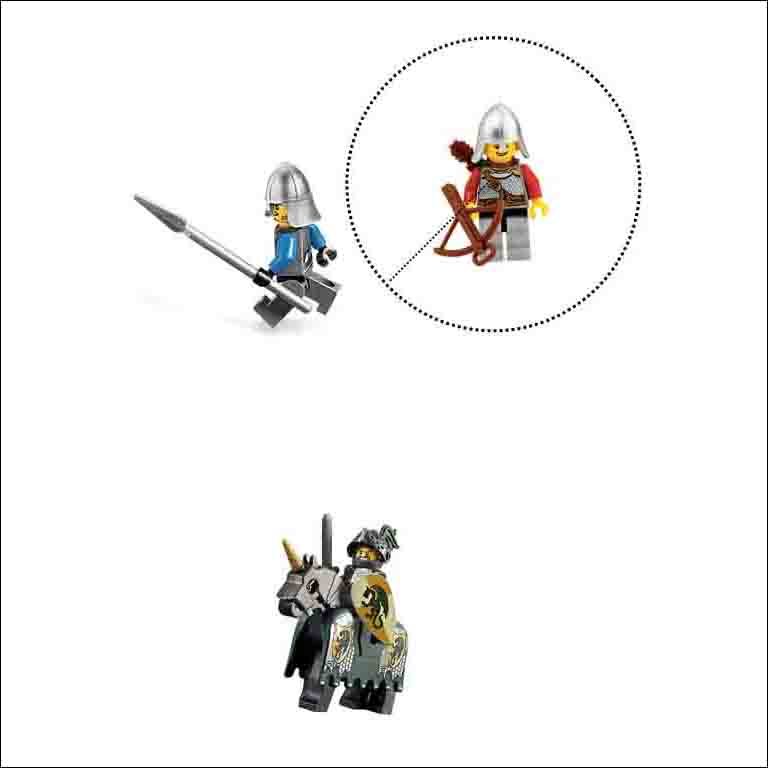
\includegraphics[width=12cm]{/Library/Server/Web/Data/Sites/webserver/PRP/distribute/CSnUsTh4/Assignment3.jpg}

	\caption{_ArcArticle_ \texttt{_Archer_}, _SmanArticle_ \texttt{_Spearman_} and _KniArticle_ \texttt{_Knight_}. The \texttt{_Archer_} and the \texttt{_Spearman_} are the two closest soldiers, so had the \texttt{_Archer_} been in range, he would have hit his target first. However, the \texttt{_Archer_} is not in range, so, actually, the \texttt{_Spearman_} wounds the \texttt{_Knight_}, because the \texttt{_Spearman_} is closer to the \texttt{_Knight_} than the \texttt{_Knight_} is to the \texttt{_Archer_}. Therefore, the \texttt{_Spearman_} wins.}

	\label{fig:assignment3}

\end{figure}

After we have determined who the winner of a battle will be, we then assume that the battle takes place. After the battle, we want to \emph{update} the position of the relevant soldiers on the battlefield based upon the winner. If the \texttt{_Archer_} wins the battle, then the wounded \texttt{_Spearman_} disappears from the battlefield (i.e. the position of the \texttt{_Spearman_} is set to some predefined value that is not on the field, such as (-1.0, -1.0)), and the \texttt{_Archer_} remains where he is. If the \texttt{_Knight_} wins, then the \texttt{_Knight_} instantly moves to the \texttt{_Archer_}'s position, and the \texttt{_Archer_} disappears. If the \texttt{_Spearman_} wins, then the \texttt{_Spearman_} instantly moves to the \texttt{_Knight_}'s location but the \texttt{_Knight_} does \emph{not} disappear from the battlefield. In all cases the third soldier is unaffected.

We want the ability to run three battles, and to understand who the winner of the battle is after each iteration.

\section{Requirements}

Write a set of classes, the use of which enables you to print who would win a battle to the terminal (i.e. which soldier would reach their target first), given the random placement of each soldier. After the winner is established, your program should move the winning and losing soldiers as instructed. This should all occur three times.

\section{Mark Scheme}

\textbf{Marks for this assignment will be awarded as follows:}

\paragraph{For 0 - 12 marks:}
		%\begin{longtable}{p{1.2cm}p{13cm}}
		%	\hline
		%	Range & Description \\
		%	\hline
			%0 - 12 & 				
								\begin{enumerate}
								\item Correctly decomposing the problem into a set of classes relevant to the problem.
								\item Using these classes to both store and provide access to all information relevant to the problem. This information should be of an appropriate type.
								\item Correctly encapsulating all information.
								\end{enumerate} %\\

\paragraph{For 12 - 15 marks}

			%\hline
			%12 - 15 & 
			All of the above, and:  \begin{enumerate}
								\item Taking the appropriate steps to ensure that all information that is required by each class is always present (e.g. every \texttt{Soldier} has a position).
								\item Positioning the soldiers on the battlefield at random locations.
								\item Providing a suitable String representation of a \texttt{Soldier}.
								\end{enumerate} %\\

\paragraph{For 15 - 20 marks}

			%\hline
			%15 - 20 & 
			All of the above, and:  \begin{enumerate}
								\item Implementing the ability for a \texttt{Soldier} to calculate the distance from himself to another \texttt{Soldier}.									\item Implementing the ability for a \texttt{Soldier} to calculate how long it would take for him to reach another \texttt{Soldier}.
								\item Computing who will win the battle (excluding the special \texttt{_Archer_} case described below).
								\end{enumerate} %\\

\paragraph{For 20 - 24 marks}
			
			%\hline
			%20 - 24 & 
			All of the above, and:  \begin{enumerate}
								\item Handling the special case in which the \texttt{_Archer_} is closest to, but still out of range of, their target.
								\item Moving each soldier to their appropriate locations after the battle is over, according to a calculation of the winner.
								\item Running three battles, and identifying three winners.
								\end{enumerate} %\\

\paragraph{For 24+ marks}
			
			%\hline
			%24+ &  
			All of the above, and:  \begin{enumerate}
							      \item Maximising efficiency through abstraction (i.e. collecting the common features of all \texttt{Soldiers}).
							      \item Computing the winner of the battle in a manner that minimises the use of conditional statements.
							      \item Returning objects from methods where appropriate, to improve the extensibility of the program.
							      \item Consistent variable name schemes and capitalisation, and consistent tabbing schemes, in order to promote reusability.
							      \item Appropriate commenting that explains your code. Javadoc is good practice, but not required.
							      \end{enumerate} %\\
			%\hline
		%\end{longtable}
		
\textbf{In addition, note that:}

\begin{enumerate}
	
	\item The mark scheme given allows for a passing mark to be achieved even if the entirety of the specification is not met.
	
	\item However, code that does not compile will receive a maximum mark of 40\%. As with all previous coursework, you must test whether your code compiles on one of the lab computers \emph{outside} of any IDE (i.e. by compiling it from the command line), even if you intend to demonstrate your code to your examiner on your own laptop.
	
	\item The mark scheme for 24 marks and above is not exhaustive. It is at the discretion of us as examiners to reward those students who demonstrate an understanding of reusability, encapsulation, abstraction and decomposition, and who produce their solutions in the most efficient manner.

	\item Exception handling and error management are not required for this assignment.
	
	\item \textbf{As in previous assignments, your final grade is based upon both the quality of your code and your ability to describe your code to your examiner.}
		
\end{enumerate}

\section{Tips}

\textbf{Tips and useful information for this assignment are as follows:}

\begin{enumerate}

	\item Do not be overwhelmed by the wording of the problem statement. Not all information needs to be captured in your program, only the information that is relevant to the requirements.
	
	\item Keep things simple. One of the model solutions to this assignment is less than 100 lines long (excluding braces, spaces and comments).
	
	\item Do not rush to a computer. This entire problem can be solved using a pen and paper. Try doing this yourself before you start to program.

	\item Start of with the easy parts of the problem first. Build what you can and what you are familiar with, and then focus on how these components can be combined and developed in order to solve the harder parts of the problem.
	
	\item Consulting the lab exercises is the \emph{best} way to gain insight into how this problem can be solved.
	
\end{enumerate}

\textbf{Once you have completed this assignment, you must place all the code you have produced into a folder, name this folder `Exercise3', compress it (to one of a .zip, .rar or .tar.gz file, no other formats) and submit it to KEATS. Please note that you should only submit plain text files with a .java extension for assessment (so no proprietary formats such as PDF or Rich Text).}

\end{document}